\documentclass[fleqn, a4paper]{article}
\usepackage[top=1.5in,bottom=1.5in,left=1.15in,right=1.15in]{geometry}
\usepackage{graphicx}
\usepackage{tikz}
\usetikzlibrary{automata, positioning, arrows}
\usepackage[export]{adjustbox}
\usepackage{float}
\usepackage{amsmath}
\usepackage{pgfplots}
\usepackage{subfig}
\pgfplotsset{compat=1.15}
\usepackage[utf8]{inputenc}

\title{EE463 Static Power Conversion I 
-Simulation Project I}
\author{Nail Tosun, Yusuf Selim Karataş}
\date{November 2018}

\usepackage{natbib}
\usepackage{graphicx}

\begin{document}

\maketitle

\section*{Question 1}
In this question we investigated the effects of different discrete step sizes on simulation in Simulink environment. Firstly we built single phase diode rectifier which connected through Turkish electrical grid ($400 V_{l-l}$ ). We connect 3 470 $\mu$F capacitors to make output voltage smoother. 
\begin{figure}[H]
  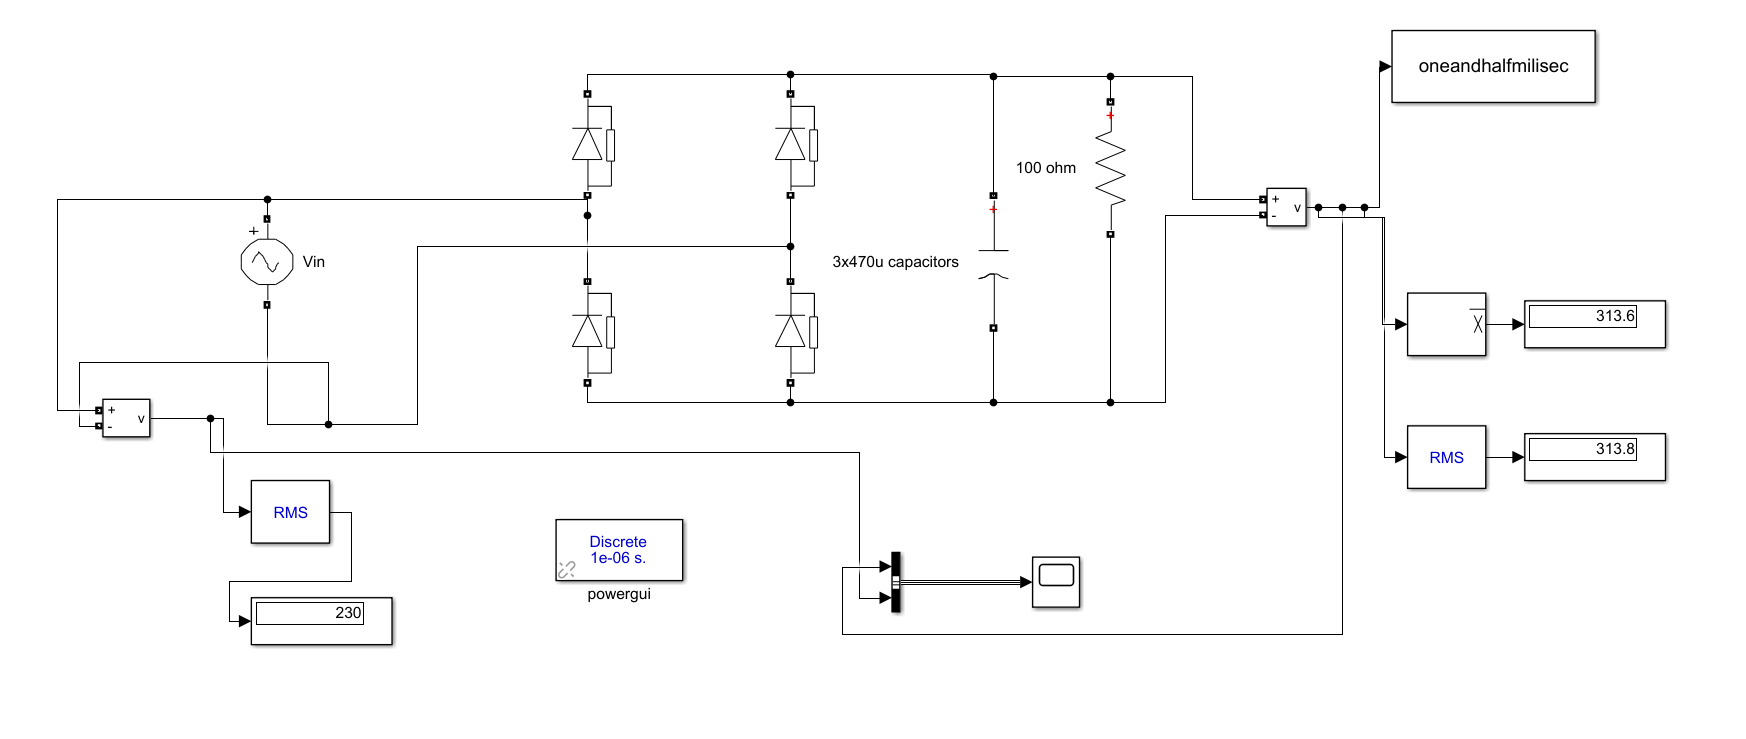
\includegraphics[width=\linewidth]{question-1-simulink-model.PNG}
  \caption{Simulink model of single phase diode rectifier}
  \label{fig:simulink2}
\end{figure}
\begin{figure}[H]
  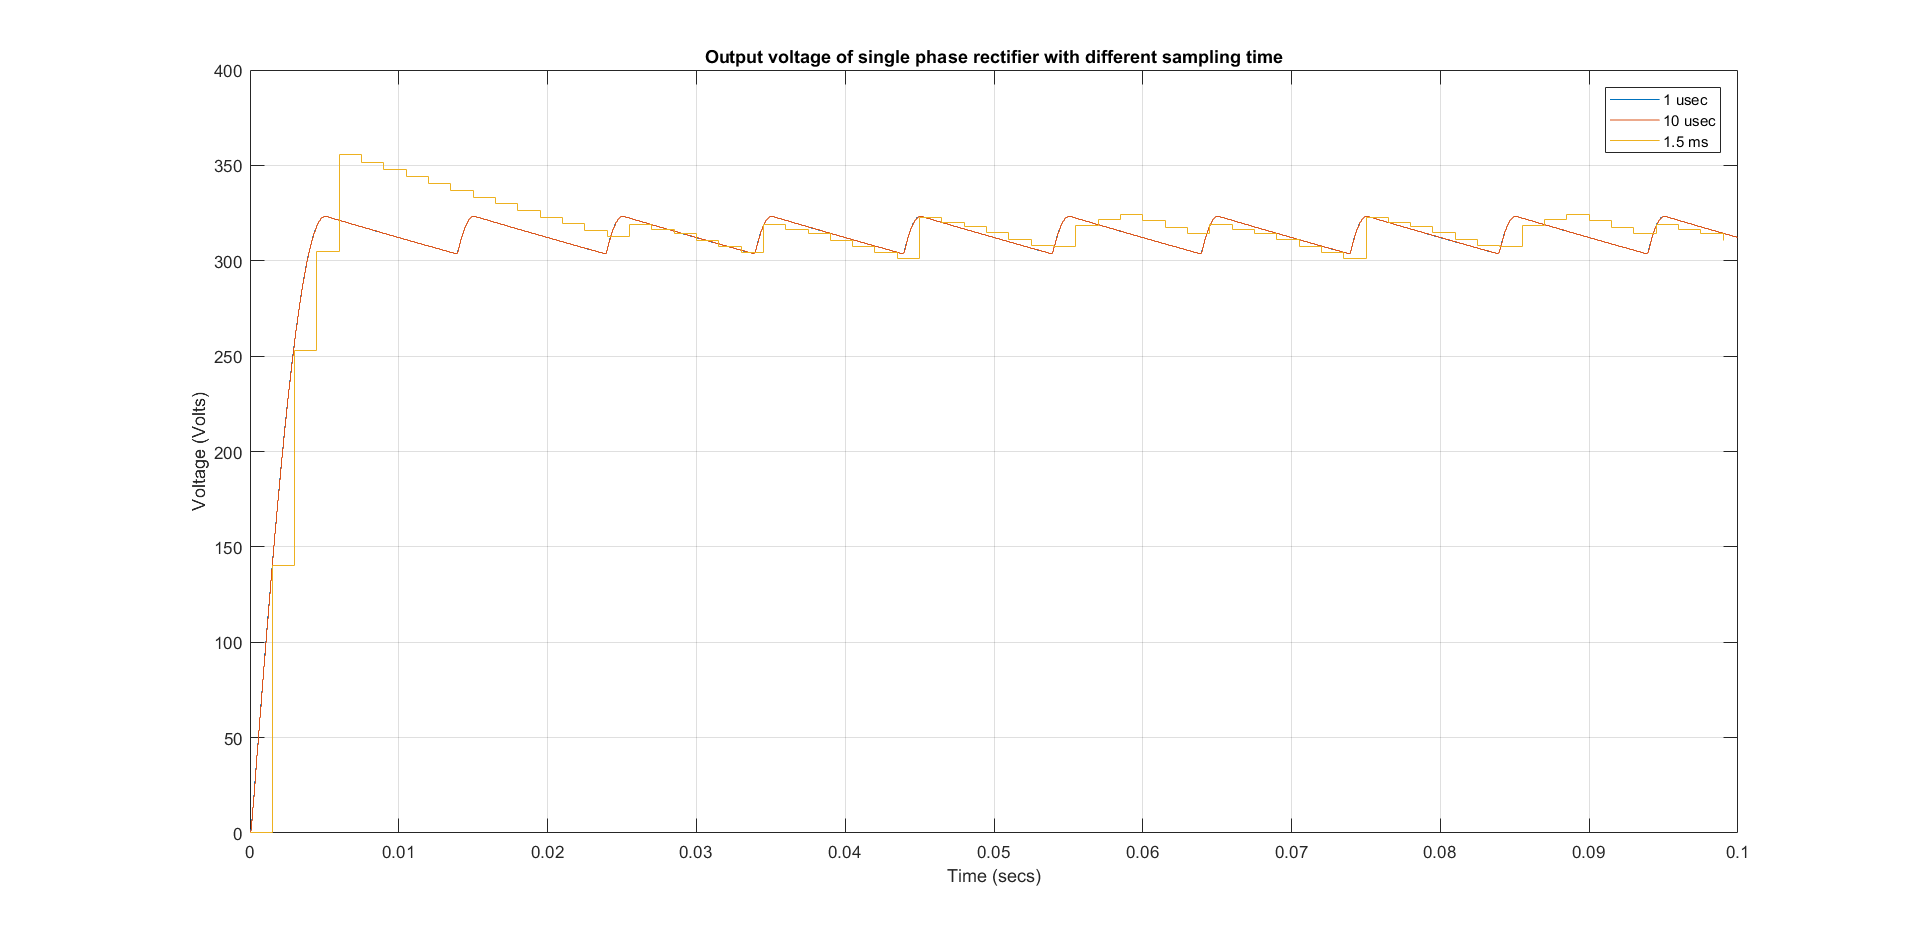
\includegraphics[width=\linewidth]{Q1_plots_different_samplings.png}
  \caption{Transients of voltage waveforms under various sampling frequencies}
  \label{fig:simulink2}
\end{figure}
\begin{figure}[H]
  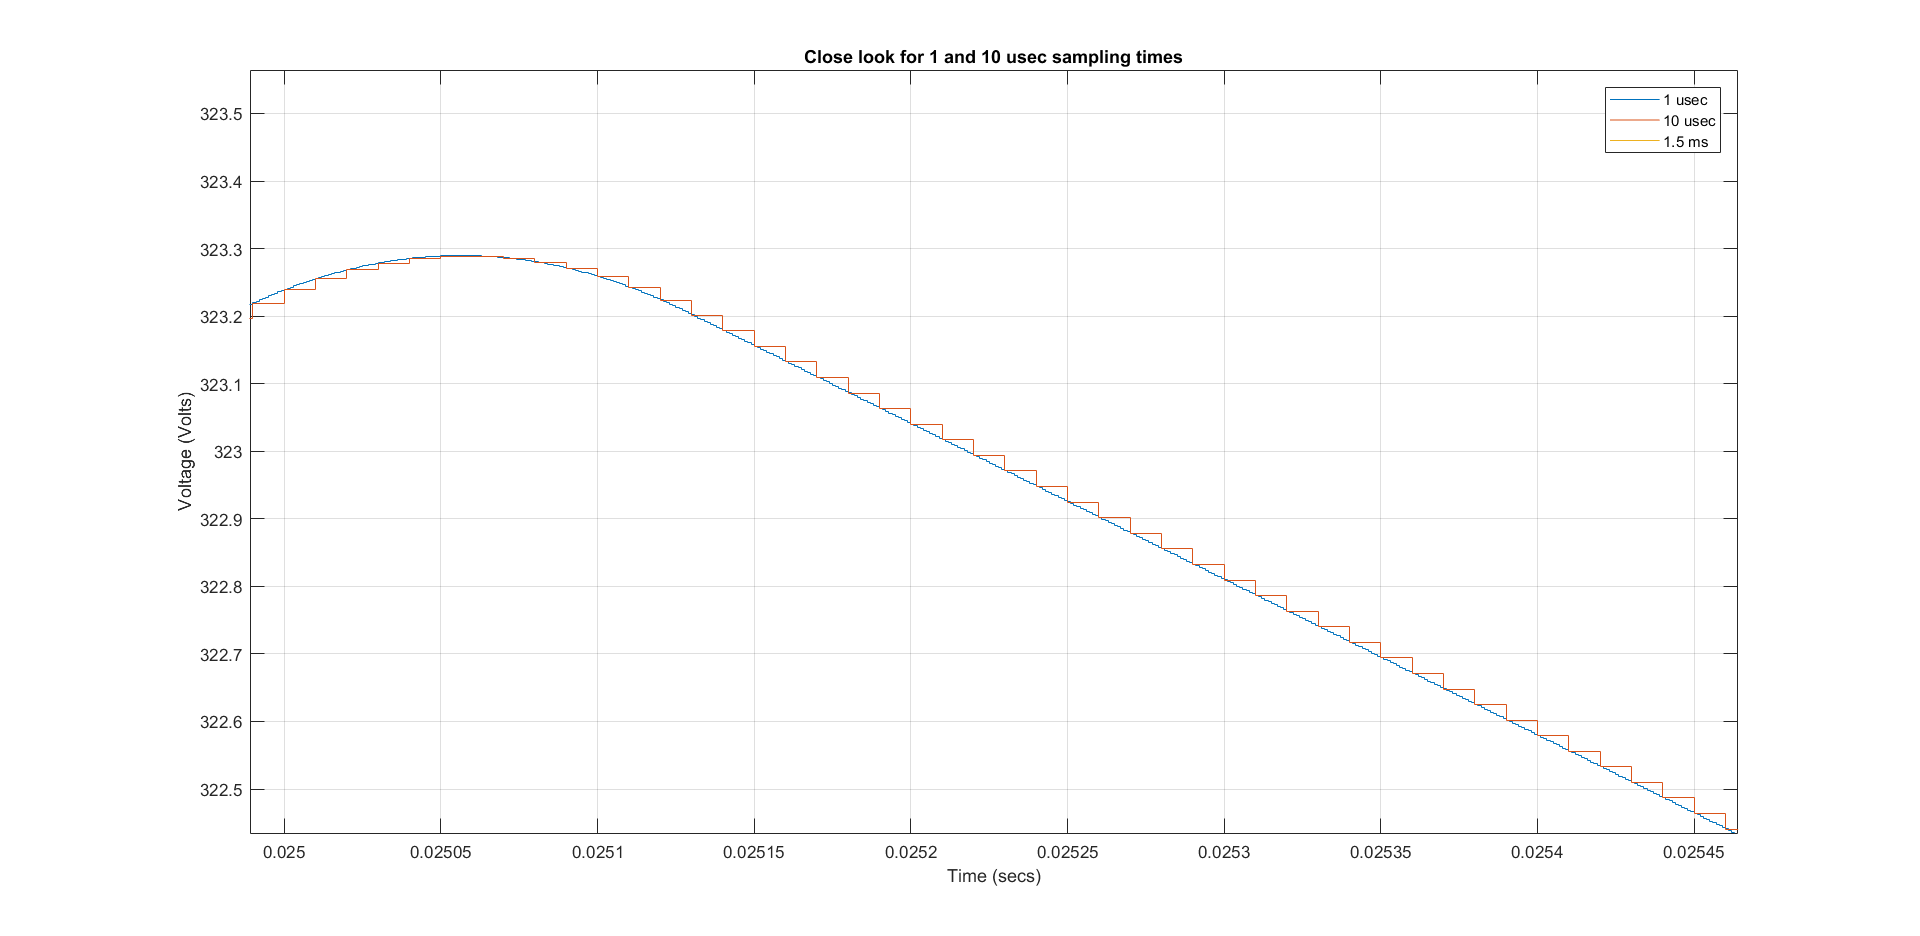
\includegraphics[width=\linewidth]{closer-look.png}
  \caption{Closer look for 1usec and 10usec to see transients}
  \label{fig:simulink2}
\end{figure}
We observed that, with large step size we lose some transients (especially at 1.5ms) but simulation time reduce since it is computationally inexpensive. With 50 Hz input signal there is no such difference between 1 $\mu$sec and 10 $\mu$sec however 1 $\mu$sec has 10 times more computational work. Therefore an engineer should do trade-off between resolution and computation time according his or her requirements.  
\section*{Question 2}
We built single phase rectifier in Simulink environment, using full-wave topology. 
\subsection*{Part 1}
Then we simulate the system different with different load configurations namely;
\begin{itemize}
	\item R = 25 ohm
	\item R = 25 ohm L = 10 mH
	\item R = 25 ohm L = 1 H
\end{itemize}
\begin{figure}[H]%
    \centering
    \subfloat[R=25 ohm]{{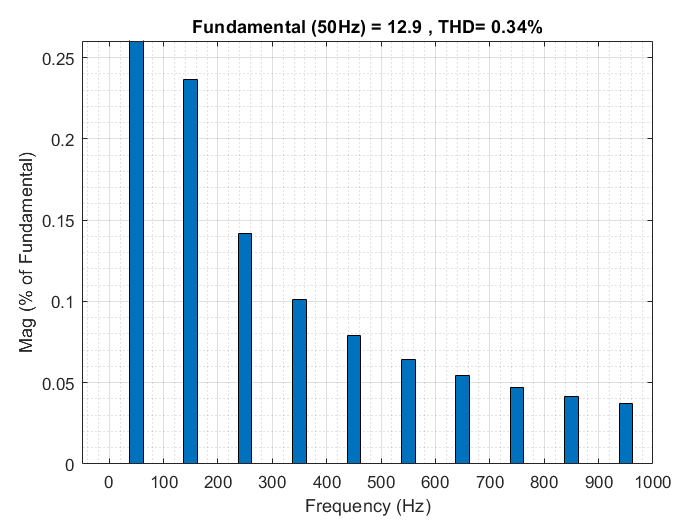
\includegraphics[width=5cm]{thd_resistive.png}}}%
    \qquad
    \subfloat[R=25 ohm L = 10 mH]{{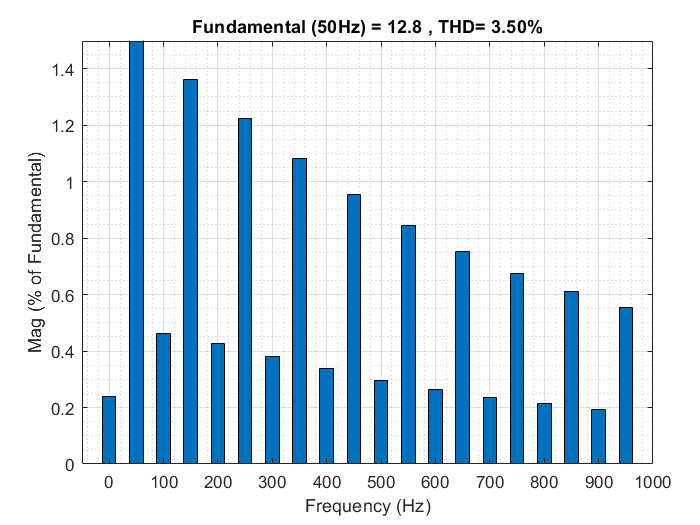
\includegraphics[width=5cm]{tenmh.png} }}%
    \qquad
    \subfloat[R=25 ohm L = 1 H]{{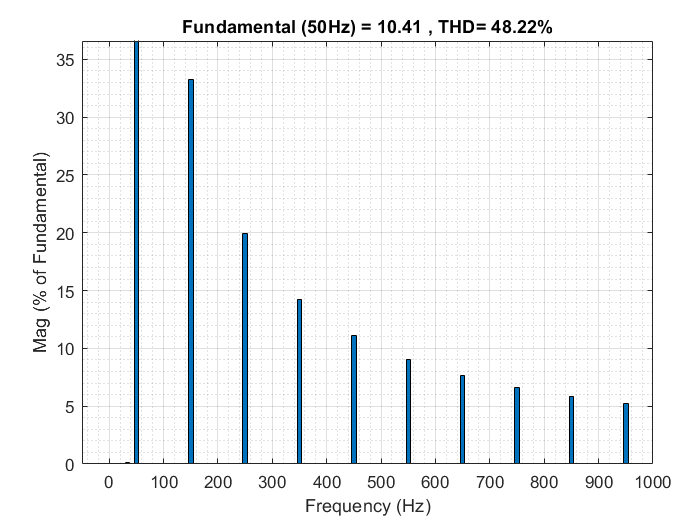
\includegraphics[width=5cm]{onehenry.png} }}%
    \caption{FFT analysis with different load configrations}%
    \label{fig:example}%
\end{figure}

\begin{table}[H]
\centering
\begin{tabular}{ll}
                      & THD      \\
R = 25 ohm            & \% 0.34  \\
R = 25 ohm L  = 10 mH & \% 3.5   \\
R = 25 ohm L = 1 H    & \% 48.22
\end{tabular}
\caption{THD with different load configrations}
\end{table} 

With only resistive load line current is sinusoidal therefore THD is very low. With increasing L load behave like current source therefore line current waveform starts to disrupt. At high inductance like 1 H the inductor behave like \textbf{ideal current source} and the line current become square wave (THD becomes \% 48). 
\subsection*{Part 2}
\subsection*{Part 3}
We added $560 \mu F $ electrolytic capacitor (565-2780-ND) decrease output voltage ripple. Some electrical parameters are given as table 1:
\begin{table}[H]
\centering
\begin{tabular}{ll}
Electrical Parameters & Average output voltage \\
Rated Voltage         & 400 V                  \\
Tolerance             & ± \%20                 \\
Capacitance           & 560 uF                 \\
Life-Time             & 2000 Hrs @ 85°C        \\
Ripple Current        & 2.69A @ 120Hz         
\end{tabular}
\caption{Electrical parameters of 565-2780-ND)}
\end{table}
We choose $560 \mu F $ electrolytic capacitors since aluminum electrolytic capacitors have high tolerance. Although $470 \mu F $ capacitors meet out performance requirements we think worst case scenario (-\%20 ) as well. Our output waveforms are;
\begin{figure}[H]
  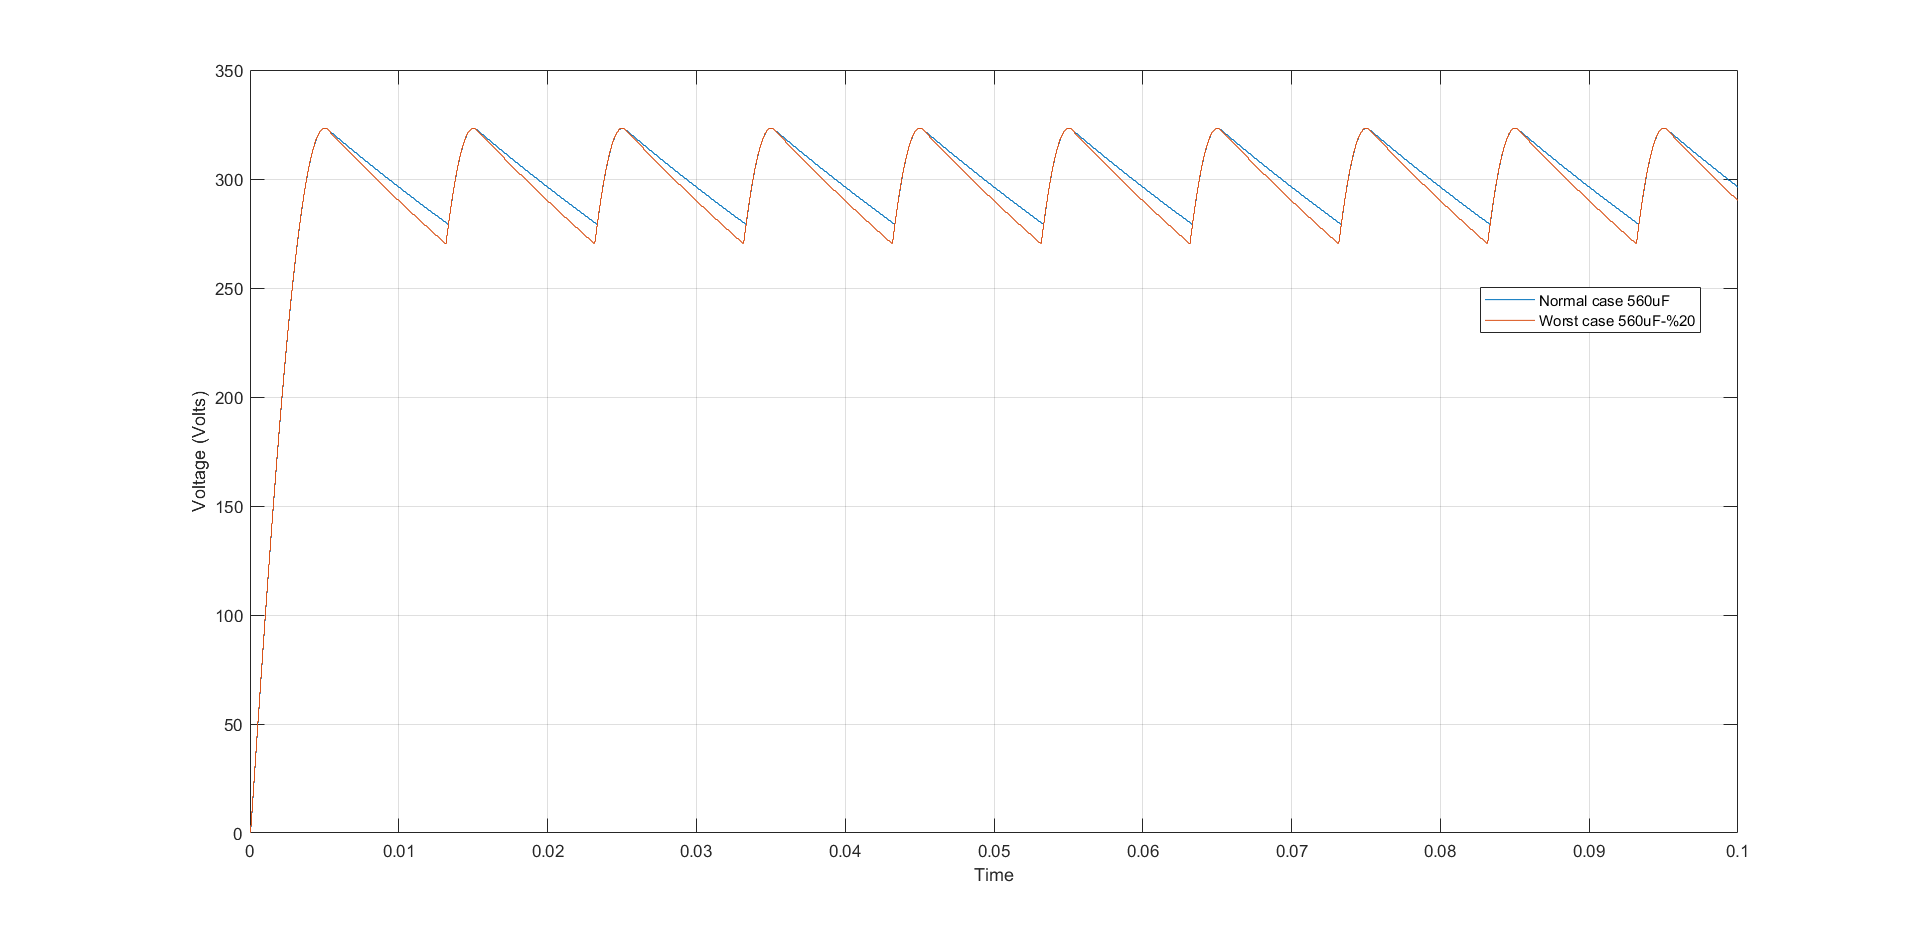
\includegraphics[width=\linewidth]{RC_load.png}
  \caption{Output waveforms both worst case and normal case scenario with RC load.}
  \label{fig:simulink2}
\end{figure}
Our ripple current (low frequency) is about 0.5 A range therefore our capacitance satisfy our ripple current requirement as well. 

\begin{figure}[H]
  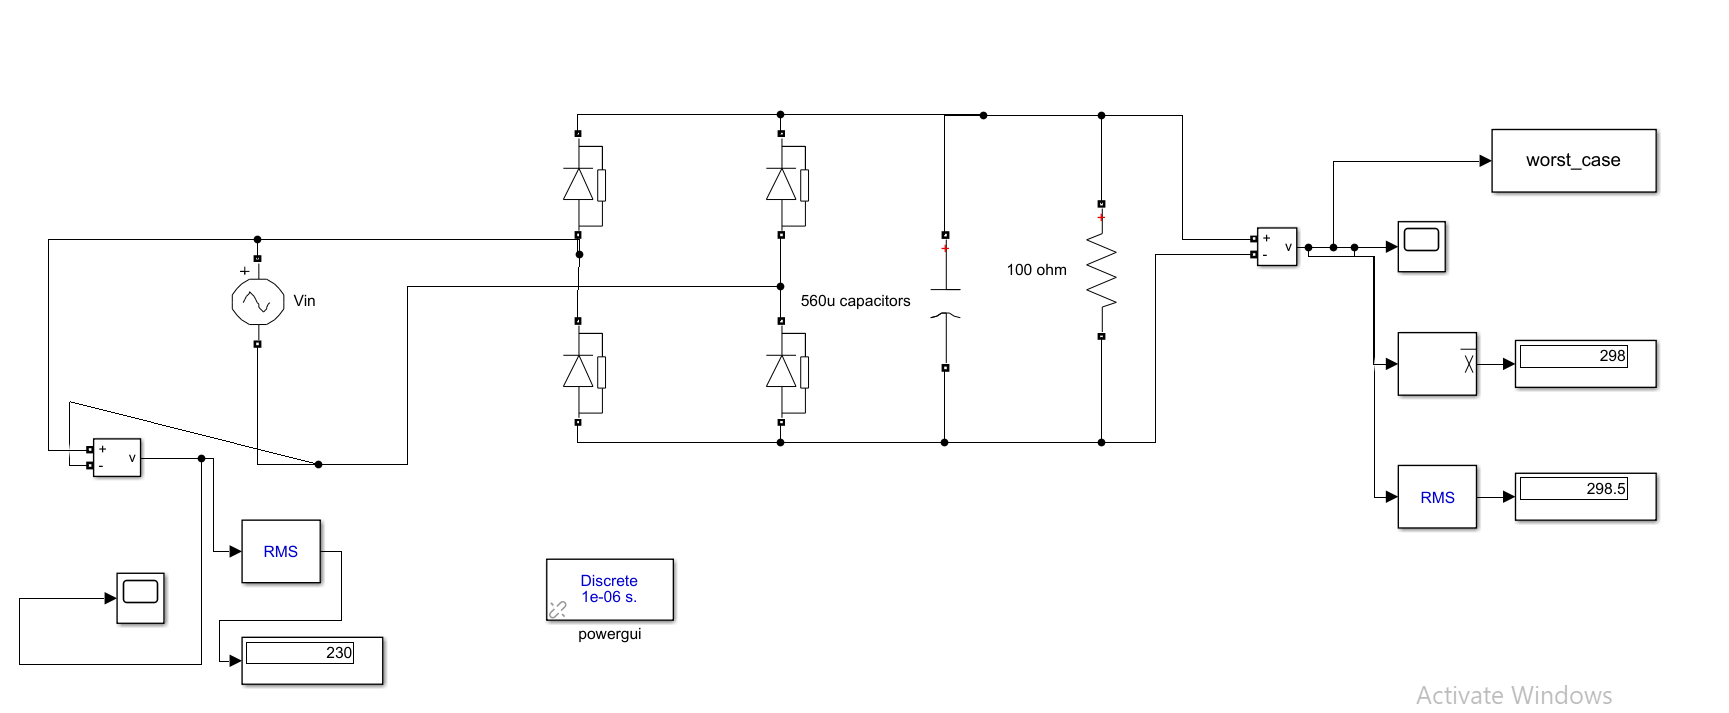
\includegraphics[width=\linewidth]{Simulink_modelRC_load.PNG}
  \caption{Simulink model of the full bridge rectifier}
  \label{fig:simulink3}
\end{figure}
Ripple voltages (both worst and normal cases) are given in following table;

\begin{table}[H]
\centering
\begin{tabular}{lll}
                       & Worst case & Normal case \\
Average output voltage & 298 V      & 302.2 V     \\
Ripple Voltage         & 53.6 V     & 44.3 V      \\
Ripple ratio           & \%18       & \%14.63    
\end{tabular}
\caption{Ripple analysis with normal and worst case scenarios}
\end{table}
\subsection*{Part 4}
At this part we observed the effect of line inductance at the source side. Since inductor current is continuous we observed \textbf{smoother current waveform} (less crest factor) with added line inductance. The output ripple voltage does not change much only the frequency increased at steady state. The effect of line inductance is mostly seen \textit{transient} output voltage. 
\begin{figure}[H]
  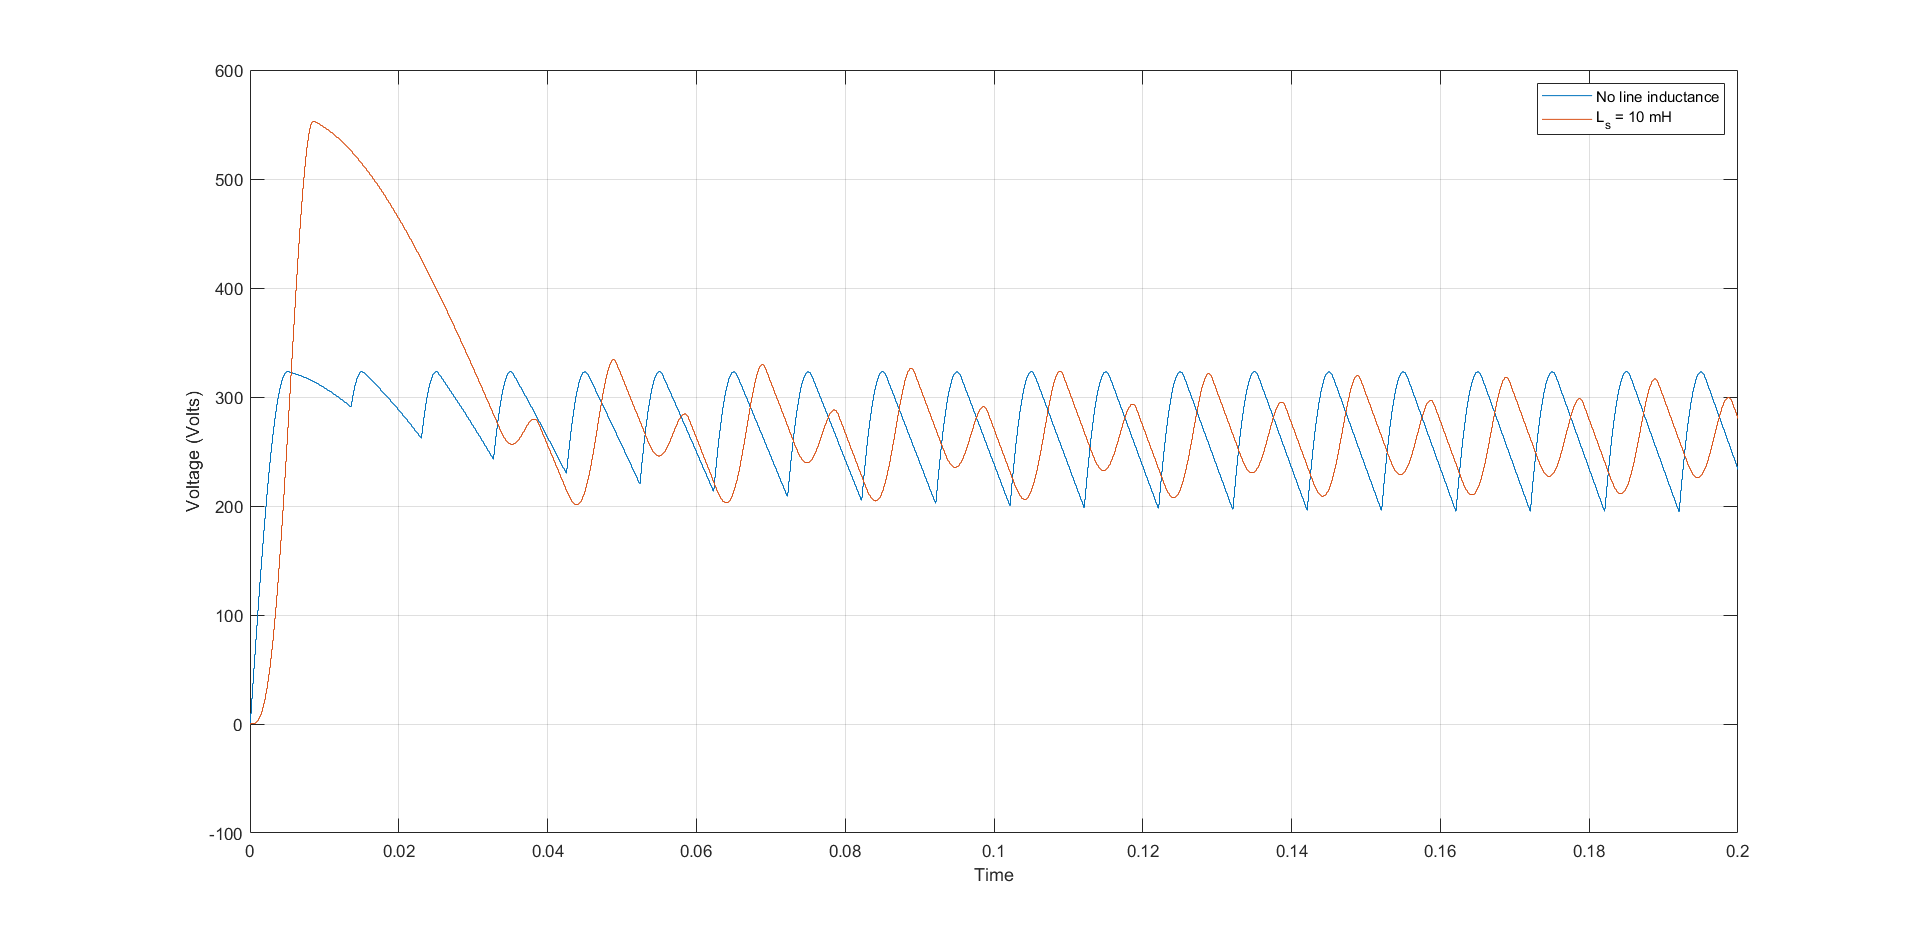
\includegraphics[width=\linewidth]{part2d.png}
  \caption{The effect of line inductance on output voltage waveform}
  \label{fig:simulink3}
\end{figure}
\begin{figure}[H]
  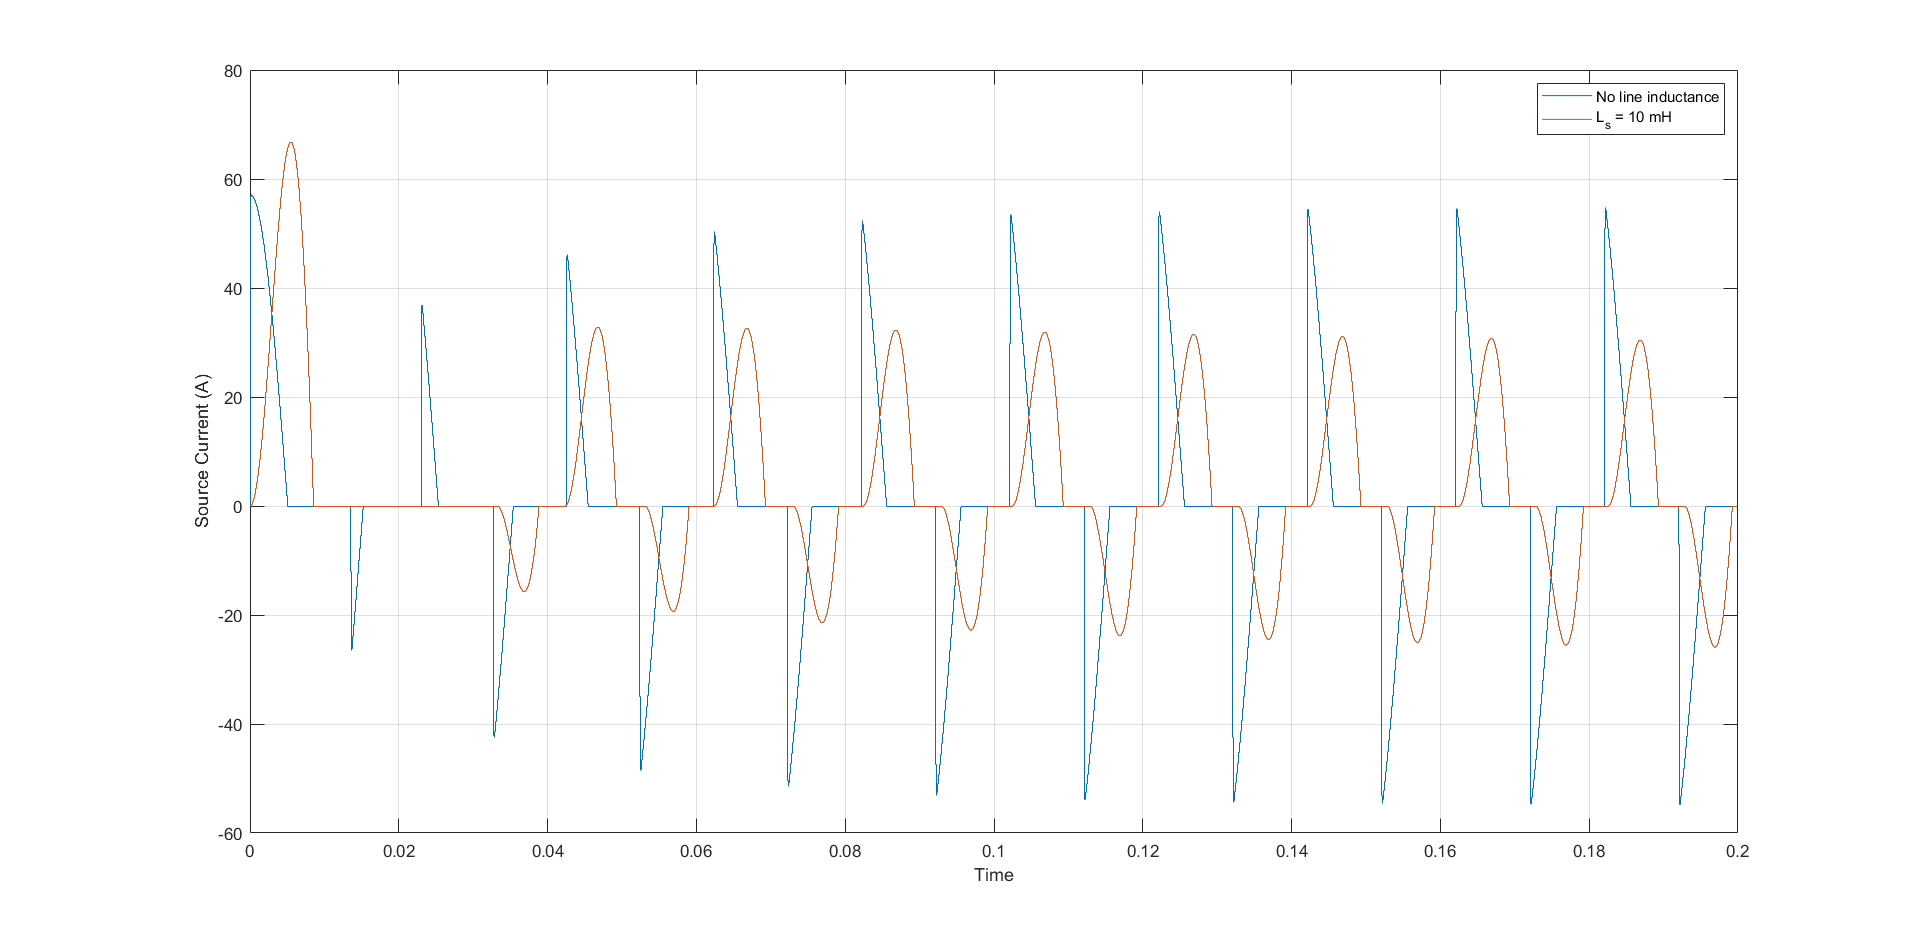
\includegraphics[width=\linewidth]{part2d2.png}
  \caption{The effect of line inductance on source current}
  \label{fig:simulink3}
\end{figure}
\subsection*{Part 5}
We choose MUR1540G with 15 A average current capability and 400 V peak repetitive reverse voltage. We make worst scenario for maximum current and peak reverse voltage. 
When line inductance 1H and R=25ohm. The maximum current 

\section*{Question 3}
In this part we have simulated three-phase diode bridge rectifier and observed power factor, THD of output current and waveforms of neutral, phase current and output voltage.
\subsection{PART 1}
\begin{figure}[H]
  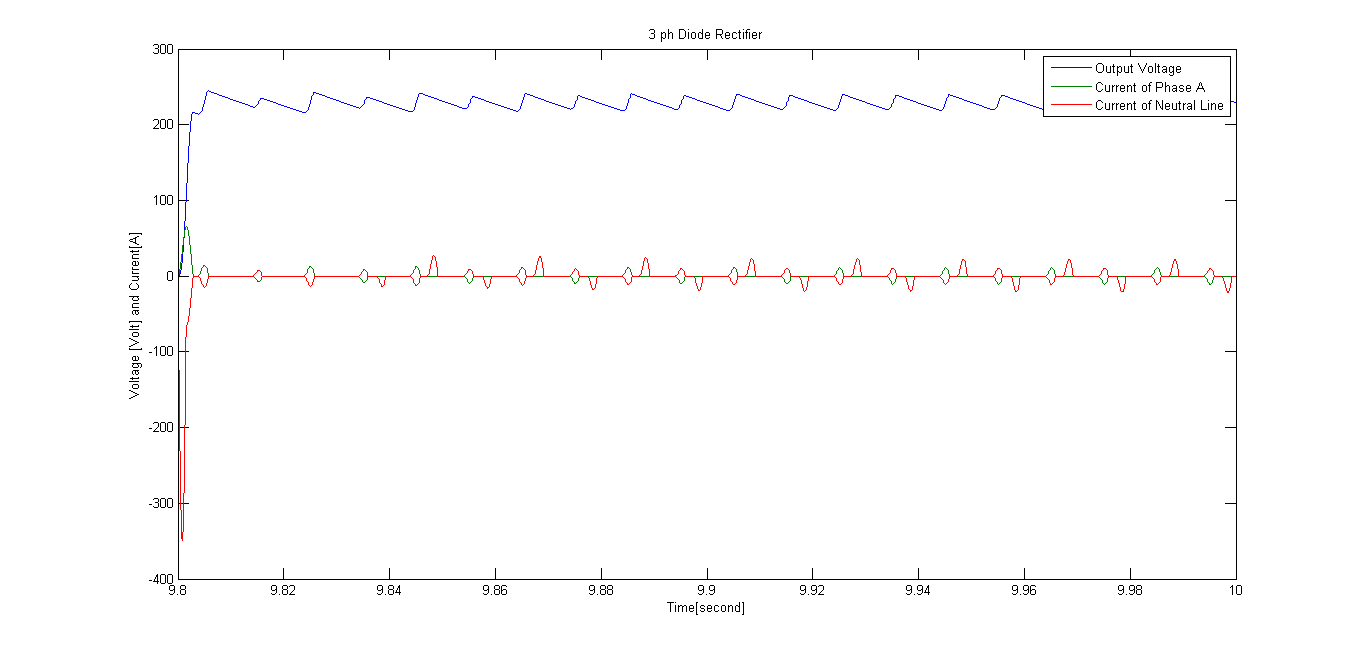
\includegraphics[width=\linewidth]{A3_1.png}
  \caption{Phase, neutral current and output voltage waveforms}
  \label{fig:simulink3}
\end{figure}

\subsection{PART 2}
\begin{figure}[H]
  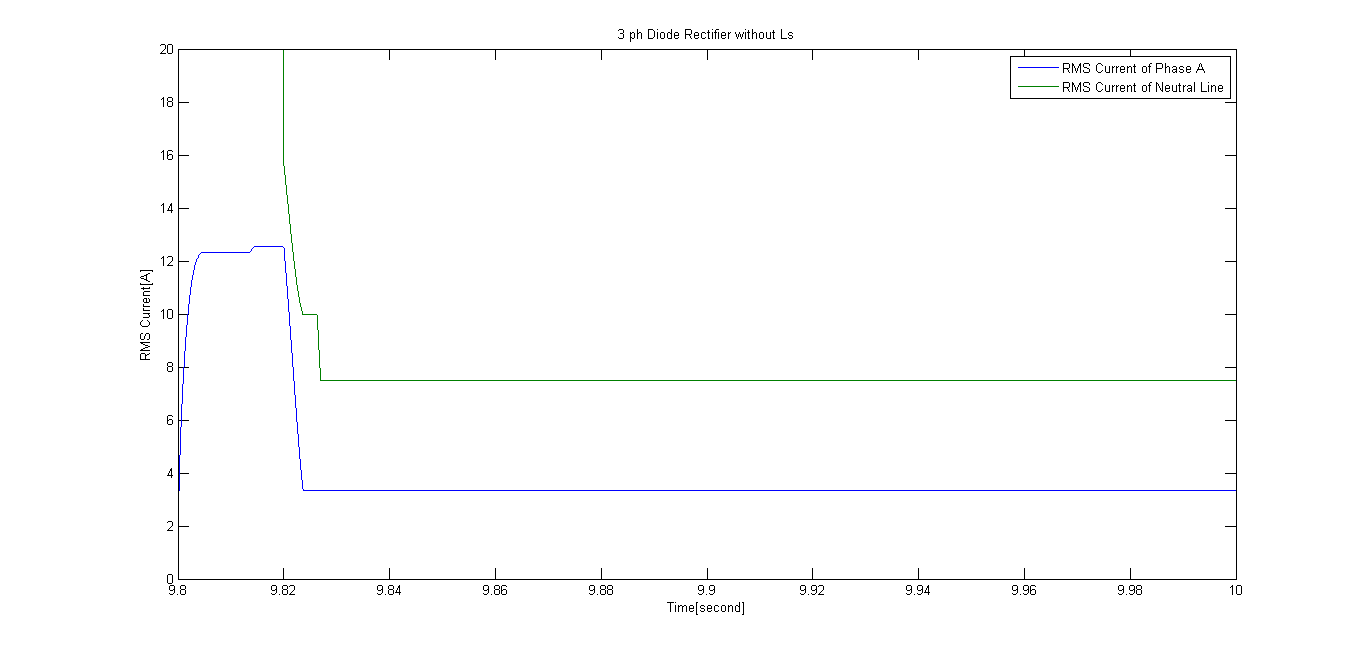
\includegraphics[width=\linewidth]{A3_3.png}
  \caption{RMS values of phase and neutral line currents}
  \label{fig:simulink3}
\end{figure}
In three-phase rectifiers each phase becomes dominant only 120 degree in each period. Since neutral line which transmits sum of the all phase currents, frequency of the neutral line current becomes three times of the grid frequency which is 50 Hz. The reason which makes neutral line current bigger than phase current is phase current's becoming 0 for 120 degree while neutral current is never 0.
\end{document}
